\documentclass[
	classe=$2^{de}$
]{évaluation}

\usepackage{tcolorbox}
\usetikzlibrary{calc}

\newcounter{LetterCounter}

\title{Évaluation : Vecteurs (rattrapage)}
\date{$1^{er}$ février 2023}
\author{}

\begin{document}

\maketitle

\begin{tcolorbox}
	Toutes les questions sont à faire sur le sujet.
\end{tcolorbox}

% 3 points ?
\begin{exercice}
	\begin{enumerate}
		\item Deux vecteurs sont égaux si ils ont la même \correctionDots{direction}, le même \correctionDots{sens} et la

		      même \correctionDots{norme}.
		\item Si deux vecteurs ont la même direction, la même norme mais des sens opposés, alors ils sont

		      \correctionDots{opposés}.
		\item \

		      \begin{minipage}{0.7\linewidth}
			      En se basant sur la figure ci-contre, répondre VRAI ou FAUX

			      à chaque question :
		      \end{minipage}
		      \begin{minipage}{0.25\linewidth}
			      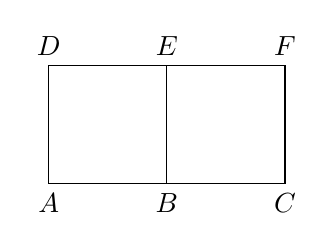
\begin{tikzpicture}[scale=1.5]
				      \coordinate (A) at (0,0);
				      \coordinate (B) at (1,0);
				      \coordinate (C) at (2,0);
				      \coordinate (D) at (0,1);
				      \coordinate (E) at (1,1);
				      \coordinate (F) at (2,1);

				      \draw (A) -- (B) -- (C) -- (F) -- (E) -- (D) -- cycle
				      (B) -- (E);
				      \node[below] at (A) {$A$};
				      \node[below] at (B) {$B$};
				      \node[below] at (C) {$C$};
				      \node[above] at (D) {$D$};
				      \node[above] at (E) {$E$};
				      \node[above] at (F) {$F$};
			      \end{tikzpicture}
		      \end{minipage}
		      \begin{multicols}{2}
			      \begin{enumerate}
				      \item $\vec{AB} = \vec{ED}$ : \correctionDots{FAUX}
				      \item $\vec{DA} = \vec{FC}$ : \correctionDots{VRAI}
				      \item $\vec{DB}$ et $\vec{EC}$ ont la même direction : \correctionDots{VRAI}
				      \item $\vec{CF}$ et $\vec{ED}$ ont la même norme : \correctionDots{VRAI}
			      \end{enumerate}
		      \end{multicols}
	\end{enumerate}
\end{exercice}

\begin{exercice}
	\begin{center}
		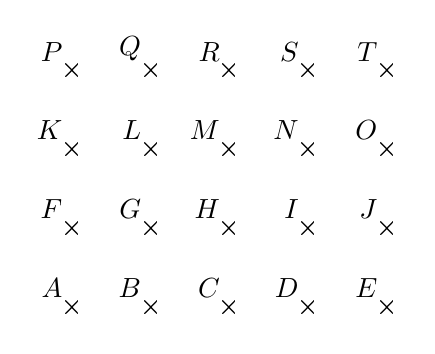
\begin{tikzpicture}
			\setcounter{LetterCounter}{0}
			\foreach \y in {0,...,3} {
					\foreach \x in {0,...,4} {
							\stepcounter{LetterCounter}
							\coordinate (\Alph{LetterCounter}) at (\x,\y);
							\node at (\Alph{LetterCounter}) {×};
							\node[above left] at (\Alph{LetterCounter}) {$\Alph{LetterCounter}$};
						}
				}
		\end{tikzpicture}
	\end{center}
	Pour chaque vecteur ci-dessous, donner \textbf{deux} de ses représentants :
	\begin{enumerate}
		\item $\vec{AB} + \vec{BG}$ : \correction{$\vec{AG}$ et $\vec{FL}$}
		\item $\frac{1}{4}\vec{FJ}$ : \correction{$\vec{FG}$ et $\vec{KL}$}
		\item $2\vec{KM} - \vec{EI}$ : \correction{$\vec{KS}$ et $\vec{FN}$}
		\item $2\vec{FR} + \frac{2}{3}\vec{RC}$ : \correction{$\vec{FT}$ et $\vec{AO}$}
	\end{enumerate}
\end{exercice}

\begin{exercice}

	Simplifier les expressions suivantes, en détaillant les calculs :
	\begin{multicols}{3}
		\begin{align*}
			A & = \vec{FE} - \vec{CD} + \vec{ED} \\
			A & =
		\end{align*}

		\columnbreak

		\begin{align*}
			B & = \vec{EA} - (\vec{EC} + \vec{ED}) + \vec{AD} \\
			B & =
		\end{align*}

		\columnbreak

		\begin{align*}
			C & = 5(\vec{u} + \vec{v}) - 2\vec{v} \\
			C & =
		\end{align*}
	\end{multicols}
\end{exercice}

\end{document}